    \section{Krožnica, krog, lok}

        


                \begin{definicija}
                        \textbf{Krožnica} je množica ravninskih točk, ki so enako oddaljene od dane točke $S$ -- \textbf{središče} krožnice. Razdalja $r$ med središčem in poljubno točko na krožnici je \textbf{polmer} ali \textbf{radij} krožnice.
                        $$\mathcal{K}=\{T; d(T,S)=r\}$$

                        \begin{figure}[H]
                            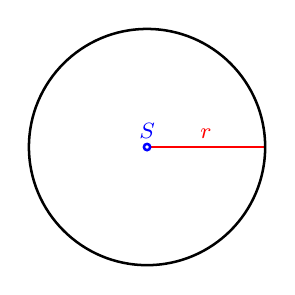
\begin{tikzpicture}
                                % \clip (0,0) rectangle (14.000000,10.000000);
                                {\footnotesize

                                % % Changing color 215 183 183
                                % \definecolor{r215g183b183}{rgb}{0.843137,0.717647,0.717647}%
                                % \color{r215g183b183}% 

                                % Changing color 255 0 0
                                \definecolor{r255g0b0}{rgb}{1.000000,0.000000,0.000000}%
                                \color{r255g0b0}% 
                                
                                % Drawing segment S R
                                \draw [line width=0.032cm] (3.040000,3.000000) -- (4.500000,3.000000);%
                                
                                % Marking point r
                                \draw (3.750000,3.000000) node [anchor=south] { $r$ };%
                                
                                % Changing color 0 0 255
                                \definecolor{r0g0b255}{rgb}{0.000000,0.000000,1.000000}%
                                \color{r0g0b255}% 
                                
                                % Marking point S by circle
                                \draw [line width=0.032cm] (3.000000,3.000000) circle (0.040000);%
                                \draw (3.000000,3.000000) node [anchor=south] { $S$ };%
                                
                                % Changing color 0 0 0
                                \definecolor{r0g0b0}{rgb}{0.000000,0.000000,0.000000}%
                                \color{r0g0b0}% 
                                
                                % Drawing circle S R
                                \draw [line width=0.032cm] (3.000000,3.000000) circle (1.500000);%
                                \color{black}
                                }
                                \end{tikzpicture}                            
                        \end{figure}

                    \end{definicija}


                    \begin{definicija}
                        \textbf{Krog} s središčem $S$ in polmerom $r$ je množica ravninskih točk, katerih oddaljenost od središča je manjša ali enaka $r$. 
                        $$\mathcal{K}=\{T; d(T,S)\leq r\}$$

                        \begin{figure}[H]
                        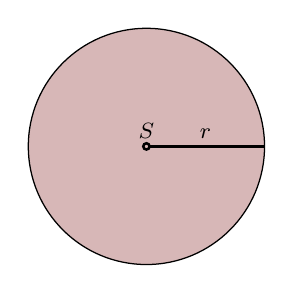
\begin{tikzpicture}
                            % \clip (0,0) rectangle (14.000000,10.000000);
                            {\footnotesize
                            
                            % Changing color 215 183 183
                            \definecolor{r215g183b183}{rgb}{0.843137,0.717647,0.717647}%
                            \color{r215g183b183}% 

                            % Changing color 255 255 0
                            % \definecolor{r255g255b0}{rgb}{1.000000,1.000000,0.000000}%
                            % \color{r255g255b0}% 
                            
                            % Filling circle s
                            \fill (3.000000,3.000000) circle (1.500000);%
                            
                            % Changing color 0 0 0
                            \definecolor{r0g0b0}{rgb}{0.000000,0.000000,0.000000}%
                            \color{r0g0b0}% 
                            
                            % Drawing circle S R
                            \draw [line width=0.016cm] (3.000000,3.000000) circle (1.500000);%
                            
                            % Drawing segment S R
                            \draw [line width=0.032cm] (3.040000,3.000000) -- (4.500000,3.000000);%
                            
                            % Marking point r
                            \draw (3.750000,3.000000) node [anchor=south] { $r$ };%
                            
                            % Marking point S by circle
                            \draw [line width=0.032cm] (3.000000,3.000000) circle (0.040000);%
                            \draw (3.000000,3.000000) node [anchor=south] { $S$ };%
                            \color{black}
                            }
                            \end{tikzpicture}
                            
                    \end{figure}

                \end{definicija}


        


        


                \begin{definicija}
                    Premico $s$, ki seka krožnico, imenujemo \textbf{sekanta} krožnice. 
                    Zveznica $CD$ njenih presečišč s krožnico je \textbf{tetiva}.
                    Presečišči $C$ in $D$ razdelita krožnico na dva \textbf{krožna loka} $\arc{CD}$ in $\arc{DC}$.
                
                \end{definicija}


                \begin{definicija}
                    Premico $t$, ki se dotika krožnice v točki $E$, imenujemo \textbf{dotikalnica} ali \textbf{tangenta} krožnice. 
                    Polmer $SE$, ki povezuje dotikališče s središčem $S$, je pravokoten na tangento.
                \end{definicija}

                \begin{definicija}
                    Točki $A$ in $B$ imenujemo \textbf{diametralni točki}, njuna zveznica je \textbf{premer} ali \textbf{diameter}.
                \end{definicija}



                    \begin{figure}[H]
                        \centering
                        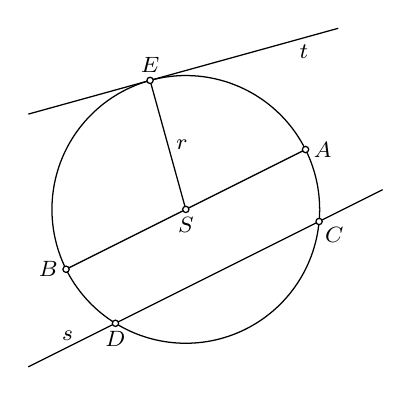
\begin{tikzpicture}
                            % \clip (0,0) rectangle (14.000000,10.000000);
                            {\footnotesize

                            % Drawing line y
                            \draw [line width=0.016cm] (4.935561,5.300000) -- (2.584843,4.649013);%
                            \draw [line width=0.016cm] (2.507744,4.627662) -- (1.000000,4.210121);%

                            % Drawing line s
                            \draw [line width=0.016cm] (1.000000,1.000000) -- (2.071165,1.535582);%
                            \draw [line width=0.016cm] (2.142719,1.571359) -- (4.657281,2.828641);%
                            \draw [line width=0.016cm] (4.728835,2.864418) -- (5.500000,3.250000);%

                            % Marking point C by circle
                            \draw [line width=0.016cm] (4.693058,2.846529) circle (0.040000);%
                            \draw (4.663058,2.876529) node [anchor=north west] { $C$ };%

                            % Marking point D by circle
                            \draw [line width=0.016cm] (2.106942,1.553471) circle (0.040000);%
                            \draw (2.106942,1.553471) node [anchor=north] { $D$ };%

                            % Drawing segment S E
                            \draw [line width=0.016cm] (2.989325,3.038549) -- (2.556969,4.599789);%

                            % Marking point E by circle
                            \draw [line width=0.016cm] (2.546294,4.638338) circle (0.040000);%
                            \draw (2.546294,4.638338) node [anchor=south] { $E$ };%

                            % Drawing circle K
                            \draw [line width=0.016cm] (4.700000,2.999999) arc (360:360:1.700000 and 1.700000) --(4.700000,3.000000) arc (0:25:1.700000 and 1.700000) -- (4.537993,3.724278);%
                            \draw [line width=0.016cm] (4.502218,3.795827) -- (4.501011,3.798102) arc (28:104:1.700000 and 1.700000) -- (2.584966,4.648559);%
                            \draw [line width=0.016cm] (2.507873,4.627209) -- (2.502968,4.625718) arc (107:205:1.700000 and 1.700000) -- (1.462007,2.275722);%
                            \draw [line width=0.016cm] (1.497782,2.204173) -- (1.498989,2.201899) arc (208:236:1.700000 and 1.700000) -- (2.073154,1.574883);%
                            \draw [line width=0.016cm] (2.141222,1.532860) -- (2.150000,1.527757) arc (240:353:1.700000 and 1.700000) -- (4.688979,2.806737);%
                            \draw [line width=0.016cm] (4.696201,2.886405) -- (4.697670,2.911028) arc (357:359:1.700000 and 1.700000) -- (4.700000,2.999999);%

                            % Marking point S by circle
                            \draw [line width=0.016cm] (3.000000,3.000000) circle (0.040000);%
                            \draw (3.000000,3.000000) node [anchor=north] { $S$ };%

                            % Marking point r
                            \draw (2.773147,3.819169) node [anchor=west] { $r$ };%

                            % Drawing segment A B
                            \draw [line width=0.016cm] (4.484749,3.742375) -- (3.035777,3.017889);%
                            \draw [line width=0.016cm] (2.964223,2.982111) -- (1.515251,2.257625);%

                            % Marking point B by circle
                            \draw [line width=0.016cm] (1.479474,2.239737) circle (0.040000);%
                            \draw (1.479474,2.239737) node [anchor=east] { $B$ };%

                            % Marking point A by circle
                            \draw [line width=0.016cm] (4.520526,3.760263) circle (0.040000);%
                            \draw (4.520526,3.760263) node [anchor=west] { $A$ };%

                            % Marking point s
                            \draw (1.500000,1.400000) node  { $s$ };%

                            % Marking point t
                            \draw (4.500000,5.000000) node  { $t$ };%
                            }
                            \end{tikzpicture}

                    \end{figure}



                
        

        
            \subsection*{Obodni in središčni kot}

            \begin{definicija}
                    \textbf{Obodni kot} nad lokom $\arc{AB}$ je kot, ki ima vrh na krožnici, kraka pa gresta skozi točki $A$ in $B$, ki določata lok.
                
                    \begin{figure}[H]
                        \centering
                        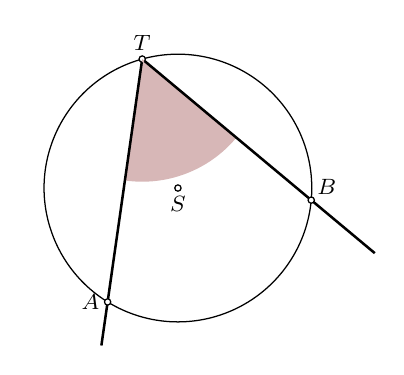
\begin{tikzpicture}
                            % \clip (0,0) rectangle (14.000000,10.000000);
                            {\footnotesize

                            % Marking point A by circle
                            \draw [line width=0.016cm] (4.693058,2.846529) circle (0.040000);%
                            \draw (4.663058,2.816529) node [anchor=south west] { $B$ };%

                            % Marking point B by circle
                            \draw [line width=0.016cm] (2.106942,1.553471) circle (0.040000);%
                            \draw (2.106942,1.553471) node [anchor=east] { $A$ };%

                            % Marking point T by circle
                            \draw [line width=0.016cm] (2.546294,4.638338) circle (0.040000);%
                            \draw (2.546294,4.638338) node [anchor=south] { $T$ };%

                            % Drawing circle K
                            \draw [line width=0.016cm] (4.700000,2.999999) arc (360:360:1.700000 and 1.700000) --(4.700000,3.000000) arc (0:104:1.700000 and 1.700000) -- (2.584966,4.648559);%
                            \draw [line width=0.016cm] (2.507873,4.627209) -- (2.502968,4.625718) arc (107:236:1.700000 and 1.700000) -- (2.073155,1.574883);%
                            \draw [line width=0.016cm] (2.141222,1.532860) -- (2.150000,1.527757) arc (240:353:1.700000 and 1.700000) -- (4.688979,2.806737);%
                            \draw [line width=0.016cm] (4.696201,2.886405) -- (4.697670,2.911028) arc (357:359:1.700000 and 1.700000) -- (4.700000,2.999999);%

                            % Marking point S by circle
                            \draw [line width=0.016cm] (3.000000,3.000000) circle (0.040000);%
                            \draw (3.000000,3.000000) node [anchor=north] { $S$ };%

                            % Changing color 215 183 183
                            \definecolor{r215g183b183}{rgb}{0.843137,0.717647,0.717647}%
                            \color{r215g183b183}% 

                            % Filling circle arc T E 58.26
                            \fill (2.546294,4.638338) -- (2.326617,3.095904) -- (2.329462,3.095502) arc (262:320:1.557998 and 1.557998) -- (3.742403,3.639998) -- cycle;%

                            % Changing color 0 0 0
                            \definecolor{r0g0b0}{rgb}{0.000000,0.000000,0.000000}%
                            \color{r0g0b0}% 

                            % Drawing line A T
                            % \draw [line width=0.032cm] (1.753556,5.300000) -- (2.515585,4.663969);%
                            \draw [line width=0.032cm] (2.577002,4.612706) -- (4.662350,2.872161);%
                            \draw [line width=0.032cm] (4.723767,2.820898) -- (5.500000,2.173011);%

                            % Drawing line B T
                            \draw [line width=0.032cm] (2.028115,1.000000) -- (2.101302,1.513870);%
                            \draw [line width=0.032cm] (2.112582,1.593071) -- (2.540654,4.598737);%
                            % \draw [line width=0.032cm] (2.551933,4.677938) -- (2.640529,5.300000);%
                            \color{black}
                            }
                            \end{tikzpicture}

                    \end{figure}

                \end{definicija}


                
                \begin{definicija}
                    \textbf{Središčni kot} nad lokom $\arc{AB}$ je kot, ki ima vrh v središču krožnice, kraka pa gresta skozi točki $A$ in $B$, ki določata lok.
                
                    \begin{figure}[H]
                        \centering
                        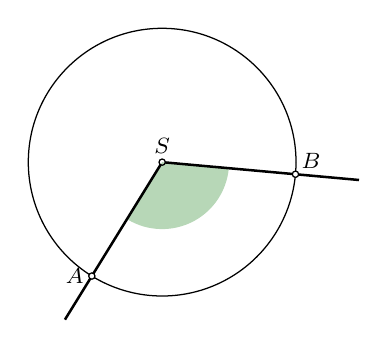
\begin{tikzpicture}
                        % \clip (0,0) rectangle (14.000000,10.000000);
                        {\footnotesize

                        % Marking point A by circle
                        \draw [line width=0.016cm] (4.693058,2.846529) circle (0.040000);%
                        \draw (4.663058,2.816529) node [anchor=south west] { $B$ };%

                        % Marking point B by circle
                        \draw [line width=0.016cm] (2.106942,1.553471) circle (0.040000);%
                        \draw (2.106942,1.553471) node [anchor=east] { $A$ };%

                        % Changing color 183 215 183
                        \definecolor{r183g215b183}{rgb}{0.717647,0.843137,0.717647}%
                        \color{r183g215b183}% 

                        % Filling circle arc S E 116.51
                        \fill (3.000000,3.000000) -- (2.553471,2.276736) -- (2.562217,2.271408) arc (239:354:0.850000 and 0.850000) -- (3.846529,2.923264) -- cycle;%

                        % Changing color 0 0 0
                        \definecolor{r0g0b0}{rgb}{0.000000,0.000000,0.000000}%
                        \color{r0g0b0}% 

                        % Drawing circle K
                        \draw [line width=0.016cm] (4.700000,2.999999) arc (360:360:1.700000 and 1.700000) --(4.700000,3.000000) arc (0:236:1.700000 and 1.700000) -- (2.073155,1.574883);%
                        \draw [line width=0.016cm] (2.141222,1.532860) -- (2.150000,1.527757) arc (240:353:1.700000 and 1.700000) -- (4.688979,2.806737);%
                        \draw [line width=0.016cm] (4.696201,2.886405) -- (4.697670,2.911028) arc (357:359:1.700000 and 1.700000) -- (4.700000,2.999999);%

                        % Marking point S by circle
                        \draw [line width=0.016cm] (3.000000,3.000000) circle (0.040000);%
                        \draw (3.000000,3.000000) node [anchor=south] { $S$ };%

                        % Changing color 0 0 0
                        \definecolor{r0g0b0}{rgb}{0.000000,0.000000,0.000000}%
                        \color{r0g0b0}% 

                        % Drawing line A S
                        % \draw [line width=0.032cm] (1.000000,3.181294) -- (2.960163,3.003611);%
                        \draw [line width=0.032cm] (3.039837,2.996389) -- (4.653222,2.850140);%
                        \draw [line width=0.032cm] (4.732895,2.842918) -- (5.500000,2.773382);%

                        % Drawing line B S
                        \draw [line width=0.032cm] (1.765240,1.000000) -- (2.085928,1.519435);%
                        \draw [line width=0.032cm] (2.127955,1.587507) -- (2.978987,2.965964);%
                        % \draw [line width=0.032cm] (3.021013,3.034036) -- (4.419974,5.300000);%
                        \color{black}
                        }
                        \end{tikzpicture}
                    \end{figure}

                \end{definicija}

                

        
            \begin{izrek}
                Nad istim lokom meri obodni kot polovico središčnega kota.

                \begin{figure}[H]
                    \centering
                    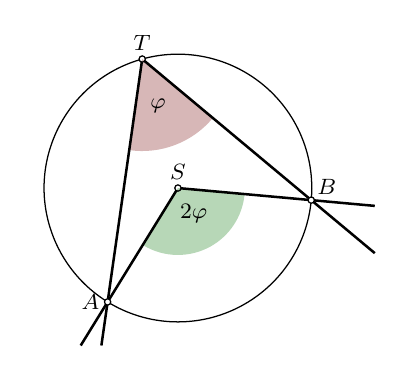
\begin{tikzpicture}
                        % \clip (0,0) rectangle (14.000000,10.000000);
                        {\footnotesize

                        % Marking point A by circle
                        \draw [line width=0.016cm] (4.693058,2.846529) circle (0.040000);%
                        \draw (4.663058,2.816529) node [anchor=south west] { $B$ };%

                        % Marking point B by circle
                        \draw [line width=0.016cm] (2.106942,1.553471) circle (0.040000);%
                        \draw (2.106942,1.553471) node [anchor=east] { $A$ };%

                        % Changing color 215 183 183
                        \definecolor{r215g183b183}{rgb}{0.843137,0.717647,0.717647}%
                        \color{r215g183b183}% 

                        % Filling circle arc T E 58.26
                        \fill (2.546294,4.638338) -- (2.381536,3.481513) -- (2.383670,3.481211) arc (262:320:1.168499 and 1.168499) -- (3.443375,3.889583) -- cycle;%

                        % Changing color 183 215 183
                        \definecolor{r183g215b183}{rgb}{0.717647,0.843137,0.717647}%
                        \color{r183g215b183}% 

                        % Filling circle arc S F 116.51
                        \fill (3.000000,3.000000) -- (2.553471,2.276736) -- (2.562217,2.271408) arc (239:354:0.850000 and 0.850000) -- (3.846529,2.923264) -- cycle;%

                        % Changing color 0 0 0
                        \definecolor{r0g0b0}{rgb}{0.000000,0.000000,0.000000}%
                        \color{r0g0b0}% 

                        % Marking point T by circle
                        \draw [line width=0.016cm] (2.546294,4.638338) circle (0.040000);%
                        \draw (2.546294,4.638338) node [anchor=south] { $T$ };%
                        \draw (2.746294,4.238338) node [anchor=north] { $\varphi$ };%

                        % Drawing circle K
                        \draw [line width=0.016cm] (4.700000,2.999999) arc (360:360:1.700000 and 1.700000) --(4.700000,3.000000) arc (0:104:1.700000 and 1.700000) -- (2.584966,4.648559);%
                        \draw [line width=0.016cm] (2.507873,4.627209) -- (2.502968,4.625718) arc (107:236:1.700000 and 1.700000) -- (2.073155,1.574883);%
                        \draw [line width=0.016cm] (2.141222,1.532860) -- (2.150000,1.527757) arc (240:353:1.700000 and 1.700000) -- (4.688979,2.806737);%
                        \draw [line width=0.016cm] (4.696201,2.886405) -- (4.697670,2.911028) arc (357:359:1.700000 and 1.700000) -- (4.700000,2.999999);%

                        % Marking point S by circle
                        \draw [line width=0.016cm] (3.000000,3.000000) circle (0.040000);%
                        \draw (3.000000,3.000000) node [anchor=south] { $S$ };%
                        \draw (3.200000,2.900000) node [anchor=north] { $2\varphi$ };%

                        % Drawing line A T
                        % \draw [line width=0.032cm] (1.753556,5.300000) -- (2.515585,4.663969);%
                        \draw [line width=0.032cm] (2.577002,4.612706) -- (4.662350,2.872161);%
                        \draw [line width=0.032cm] (4.723767,2.820898) -- (5.500000,2.173011);%

                        % Drawing line B T
                        \draw [line width=0.032cm] (2.028115,1.000000) -- (2.101302,1.513870);%
                        \draw [line width=0.032cm] (2.112582,1.593071) -- (2.540654,4.598737);%
                        % \draw [line width=0.032cm] (2.551933,4.677938) -- (2.640529,5.300000);%

                        % Drawing line A S
                        % \draw [line width=0.032cm] (1.000000,3.181294) -- (2.960163,3.003611);%
                        \draw [line width=0.032cm] (3.039837,2.996389) -- (4.653222,2.850140);%
                        \draw [line width=0.032cm] (4.732895,2.842918) -- (5.500000,2.773382);%

                        % Drawing line B S
                        \draw [line width=0.032cm] (1.765240,1.000000) -- (2.085928,1.519435);%
                        \draw [line width=0.032cm] (2.127955,1.587507) -- (2.978987,2.965964);%
                        % \draw [line width=0.032cm] (3.021013,3.034036) -- (4.419974,5.300000);%
                        \color{black}
                        }
                        \end{tikzpicture}

                \end{figure}
            \end{izrek}

            \begin{izrek}
                Vsi obodni koti nad istim lokom so enaki/skladni.
            \end{izrek}
        


        
            \begin{izrek}[Talesov izrek o kotu v polkrogu]
                Če je osnovnica trikotnika premer kroga in tretje oglišče trikotnika leži na krožnici, je trikotnik pravokoten.
            
                \begin{figure}[H]
                    \centering
                    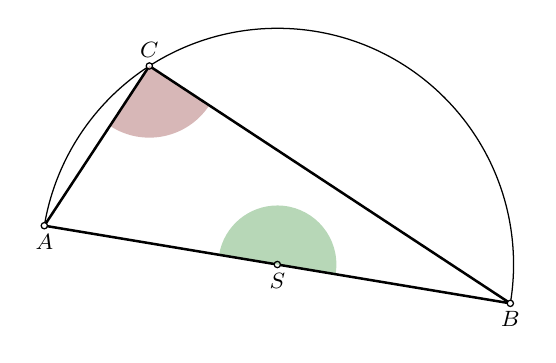
\begin{tikzpicture}
                    % \clip (0,0) rectangle (14.000000,10.000000);
                    {\footnotesize

                    % Marking point A by circle
                    \draw [line width=0.016cm] (1.040818,2.493197) circle (0.040000);%
                    \draw (1.040818,2.493197) node [anchor=north] { $A$ };%

                    % Marking point B by circle
                    \draw [line width=0.016cm] (6.959182,1.506803) circle (0.040000);%
                    \draw (6.959182,1.506803) node [anchor=north] { $B$ };%

                    % Changing color 215 183 183
                    \definecolor{r215g183b183}{rgb}{0.843137,0.717647,0.717647}%
                    \color{r215g183b183}% 

                    % Filling circle arc C E 90.00
                    \fill (2.374663,4.521563) -- (1.874471,3.760926) -- (1.878843,3.758068) arc (237:326:0.910363 and 0.910363) -- (3.135300,4.021371) -- cycle;%

                    % Changing color 183 215 183
                    \definecolor{r183g215b183}{rgb}{0.717647,0.843137,0.717647}%
                    \color{r183g215b183}% 

                    % Filling circle arc S F -180.00
                    \fill (4.000000,2.000000) -- (4.739795,1.876701) -- (4.740766,1.882674) arc (351:360:0.750000 and 0.750000) --(4.750000,2.000000) arc (0:170:0.750000 and 0.750000) -- (3.260205,2.123299) -- cycle;%

                    % Changing color 0 0 0
                    \definecolor{r0g0b0}{rgb}{0.000000,0.000000,0.000000}%
                    \color{r0g0b0}% 

                    % Marking point C by circle
                    \draw [line width=0.016cm] (2.374663,4.521563) circle (0.040000);%
                    \draw (2.374663,4.521563) node [anchor=south] { $C$ };%

                    % Drawing arc S B 180.00
                    \draw [line width=0.016cm] (6.965494,1.546301) -- (6.970804,1.582480) arc (352:360:3.000000 and 3.000000) --(7.000000,2.000000) arc (0:122:3.000000 and 3.000000) -- (2.408427,4.543009);%
                    \draw [line width=0.016cm] (2.341187,4.499668) -- (2.322422,4.487113) arc (124:169:3.000000 and 3.000000) -- (1.047657,2.532608);%

                    % Marking point S by circle
                    \draw [line width=0.016cm] (4.000000,2.000000) circle (0.040000);%
                    \draw (4.000000,2.000000) node [anchor=north] { $S$ };%

                    % Drawing line A C
                    % \draw [line width=0.032cm] (3.346877,6.000000) -- (2.396640,4.554984);%
                    \draw [line width=0.032cm] (2.352685,4.488141) -- (1.062796,2.526618);%
                    % \draw [line width=0.032cm] (1.018841,2.459776) -- (1.000000,2.431125);%

                    % Drawing line B C
                    % \draw [line width=0.032cm] (1.000000,5.425535) -- (2.341241,4.543540);%
                    \draw [line width=0.032cm] (2.408084,4.499585) -- (6.925760,1.528781);%
                    % \draw [line width=0.032cm] (6.992603,1.484825) -- (7.500000,1.151163);%

                    % Drawing line A S
                    % \draw [line width=0.032cm] (1.000000,2.500000) -- (1.001362,2.499773);%
                    \draw [line width=0.032cm] (1.080274,2.486621) -- (3.960544,2.006576);%
                    \draw [line width=0.032cm] (4.039456,1.993424) -- (6.919726,1.513379);%
                    % \draw [line width=0.032cm] (6.998638,1.500227) -- (7.500000,1.416667);%

                    % % Drawing line B S
                    % \draw [line width=0.032cm] (1.000000,2.500000) -- (1.001362,2.499773);%
                    % \draw [line width=0.032cm] (1.080274,2.486621) -- (3.960544,2.006576);%
                    % \draw [line width=0.032cm] (4.039456,1.993424) -- (6.919726,1.513379);%
                    % \draw [line width=0.032cm] (6.998638,1.500227) -- (7.500000,1.416667);%
                    \color{black}
                    }
                    \end{tikzpicture}
                \end{figure}
            \end{izrek}

                Kotu v polkrogu pravimo tudi obodni kot nad premerom kroga.
        


        
            \begin{naloga}
                Vsota velikosti središčnega in obodnega kota nad istim lokom je $174^\circ$. 
                Koliko merita središčni in obodni kot?
            \end{naloga}

            \begin{naloga}
                Središčni kot je za $64^\circ$ večji od obodnega kota nad istim lokom. 
                Izračunajte velikosti obeh kotov.
            \end{naloga}

            \begin{naloga}
                Krožnica je razdeljena s tremi točkami $A$, $B$ in $C$ na tri loke $AB$, $BC$ in $CA$, 
                ki so po dolžini v razmerju $2:7:9$.
                Izračunajte velikosti središčnih kotov, ki pripadajo tem lokom, ter notranjih kotov trikotnika $\triangle ABC$.
                Pomagajte si s skico.
            \end{naloga}
        


        
            \begin{naloga}
                Izračunajte vrednost neznanke $x$, če sta premici skozi točki $A$ in $T$ ter $B$ in $T$ tangenti na krožnico.

                \begin{figure}[H]
                    \centering
                    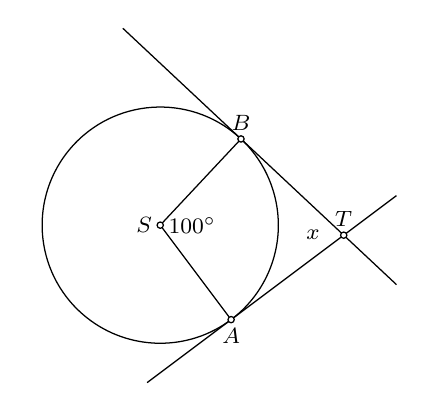
\begin{tikzpicture}
                    % \clip (0,0) rectangle (14.000000,10.000000);
                    {\footnotesize

                    % Drawing circle K
                    \draw [line width=0.016cm] (4.500000,3.000000) arc (360:360:1.500000 and 1.500000) --(4.500000,3.000000) arc (0:45:1.500000 and 1.500000) -- (4.054311,4.066972);%
                    \draw [line width=0.016cm] (3.995932,4.121659) -- (3.984089,4.132064) arc (49:305:1.500000 and 1.500000) -- (3.867682,1.776429);%
                    \draw [line width=0.016cm] (3.931677,1.824424) -- (3.943980,1.834281) arc (309:360:1.500000 and 1.500000);%

                    % Marking point A by circle
                    \draw [line width=0.016cm] (3.900000,1.800000) circle (0.040000);%
                    \draw (3.900000,1.800000) node [anchor=north] { $A$ };%

                    % Marking point S by circle
                    \draw [line width=0.016cm] (3.000000,3.000000) circle (0.040000);%
                    \draw (3.000000,3.000000) node [anchor=east] { $S$ };%
                    \draw (3.000000,3.000000) node [anchor=west] { $100^\circ$ };%

                    % Marking point B by circle
                    \draw [line width=0.016cm] (4.025486,4.094705) circle (0.040000);%
                    \draw (4.025486,4.094705) node [anchor=south] { $B$ };%

                    % Drawing segment S B
                    \draw [line width=0.016cm] (3.027346,3.029192) -- (3.998140,4.065513);%

                    % Drawing segment S A
                    \draw [line width=0.016cm] (3.024000,2.968000) -- (3.876000,1.832000);%

                    % Drawing line ta
                    \draw [line width=0.016cm] (2.833333,1.000000) -- (3.868000,1.776000);%
                    \draw [line width=0.016cm] (3.932000,1.824000) -- (5.298104,2.848578);%
                    \draw [line width=0.016cm] (5.362104,2.896578) -- (6.000000,3.375000);%

                    % Drawing line tb
                    \draw [line width=0.016cm] (2.525336,5.500000) -- (3.996294,4.122051);%
                    \draw [line width=0.016cm] (4.054678,4.067358) -- (5.300912,2.899924);%
                    \draw [line width=0.016cm] (5.359296,2.845232) -- (6.000000,2.245040);%

                    % Marking point T by circle
                    \draw [line width=0.016cm] (5.330104,2.872578) circle (0.040000);%
                    \draw (5.330104,2.872578) node [anchor=south] { $T$ };%
                    \draw (5.130104,2.872578) node [anchor=east] { $x$ };%
                    }
                    \end{tikzpicture} ~~~~~~
                    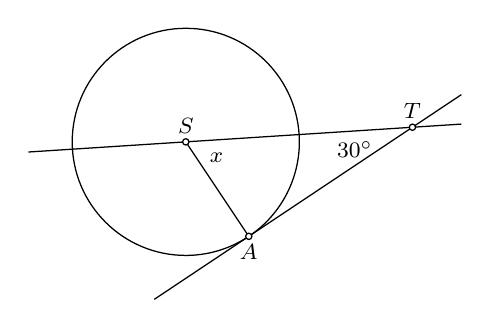
\begin{tikzpicture}
                    % \clip (0,0) rectangle (14.000000,10.000000);
                    {\footnotesize

                    % Drawing circle K
                    \draw [line width=0.016cm] (4.442221,3.000000) arc (360:360:1.442221 and 1.442221) --(4.442221,3.000000) arc (0:302:1.442221 and 1.442221) -- (3.766413,1.778275);%
                    \draw [line width=0.016cm] (3.832971,1.822647) -- (3.847716,1.833219) arc (306:360:1.442221 and 1.442221);%

                    % Marking point A by circle
                    \draw [line width=0.016cm] (3.800000,1.800000) circle (0.040000);%
                    \draw (3.800000,1.800000) node [anchor=north] { $A$ };%

                    % Marking point S by circle
                    \draw [line width=0.016cm] (3.000000,3.000000) circle (0.040000);%
                    \draw (3.000000,3.000000) node [anchor=south] { $S$ };%
                    \draw (3.200000,2.800000) node [anchor=west] { $x$ };%

                    % Drawing segment S A
                    \draw [line width=0.016cm] (3.022188,2.966718) -- (3.777812,1.833282);%

                    % Drawing line ta
                    \draw [line width=0.016cm] (2.600000,1.000000) -- (3.766718,1.777812);%
                    \draw [line width=0.016cm] (3.833282,1.822188) -- (5.845179,3.163452);%
                    \draw [line width=0.016cm] (5.911743,3.207828) -- (6.500000,3.600000);%

                    % Marking point T by circle
                    \draw [line width=0.016cm] (5.878461,3.185640) circle (0.040000);%
                    \draw (5.878461,3.185640) node [anchor=south] { $T$ };%
                    \draw (5.478461,2.900000) node [anchor=east] { $30^\circ$ };%

                    % Drawing line S T
                    \draw [line width=0.016cm] (1.000000,2.871014) -- (2.960083,2.997426);%
                    \draw [line width=0.016cm] (3.039917,3.002574) -- (5.838544,3.183066);%
                    \draw [line width=0.016cm] (5.918378,3.188215) -- (6.500000,3.225725);%
                    }
                    \end{tikzpicture}

                \end{figure}
            \end{naloga}

        


        
            \begin{naloga}
                Izračunajte vrednost neznanke $x$, če sta premici skozi točki $A$ in $T$ ter $B$ in $T$ tangenti na krožnico.

                \begin{figure}[H]
                    \centering
                    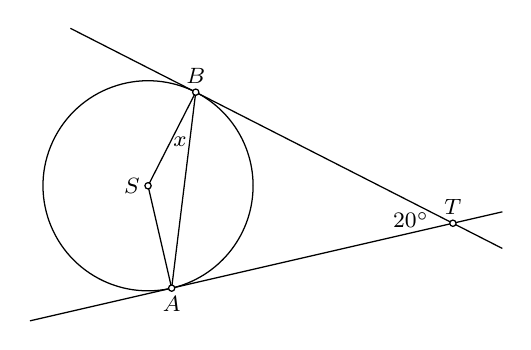
\begin{tikzpicture}
                    % \clip (0,0) rectangle (14.000000,10.000000);
                    {\footnotesize

                    % Drawing circle K
                    \draw [line width=0.016cm] (4.334166,3.000000) arc (360:360:1.334166 and 1.334166) --(4.334166,3.000000) arc (0:61:1.334166 and 1.334166) -- (3.641173,4.169999);%
                    \draw [line width=0.016cm] (3.569904,4.206321) -- (3.563843,4.209165) arc (65:281:1.334166 and 1.334166) -- (3.260893,1.691591);%
                    \draw [line width=0.016cm] (3.338836,1.709578) -- (3.345307,1.711294) arc (285:360:1.334166 and 1.334166);%

                    % Marking point A by circle
                    \draw [line width=0.016cm] (3.300000,1.700000) circle (0.040000);%
                    \draw (3.300000,1.700000) node [anchor=north] { $A$ };%

                    % Marking point S by circle
                    \draw [line width=0.016cm] (3.000000,3.000000) circle (0.040000);%
                    \draw (3.000000,3.000000) node [anchor=east] { $S$ };%

                    % Marking point B by circle
                    \draw [line width=0.016cm] (3.605811,4.188694) circle (0.040000);%
                    \draw (3.605811,4.188694) node [anchor=south] { $B$ };%
                    \draw (3.405811,3.728694) node [anchor=north] { $x$ };%

                    % Drawing segment S B
                    \draw [line width=0.016cm] (3.018163,3.035639) -- (3.587648,4.153055);%

                    % Drawing segment S A
                    \draw [line width=0.016cm] (3.008994,2.961024) -- (3.291006,1.738976);%

                    % Drawing line ta
                    \draw [line width=0.016cm] (1.500000,1.284615) -- (3.261024,1.691006);%
                    \draw [line width=0.016cm] (3.338976,1.708994) -- (6.832744,2.515249);%
                    \draw [line width=0.016cm] (6.910696,2.533237) -- (7.500000,2.669231);%

                    % Drawing line tb
                    \draw [line width=0.016cm] (2.013903,5.000000) -- (3.570172,4.206857);%
                    \draw [line width=0.016cm] (3.641449,4.170531) -- (6.836081,2.542406);%
                    \draw [line width=0.016cm] (6.907359,2.506080) -- (7.500000,2.204044);%

                    % Marking point T by circle
                    \draw [line width=0.016cm] (6.871720,2.524243) circle (0.040000);%
                    \draw (6.871720,2.524243) node [anchor=south] { $T$ };%
                    \draw (6.671720,2.564243) node [anchor=east] { $20^\circ$ };%

                    % Drawing segment A B
                    \draw [line width=0.016cm] (3.304879,1.739701) -- (3.600932,4.148993);%
                    }
                    \end{tikzpicture}~~~~~~
                    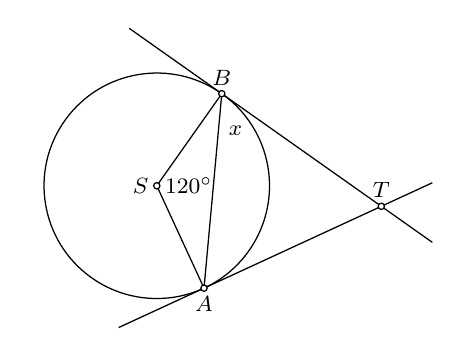
\begin{tikzpicture}
                    % \clip (0,0) rectangle (14.000000,10.000000);
                    {\footnotesize

                    % Drawing circle K
                    \draw [line width=0.016cm] (4.431782,3.000000) arc (360:360:1.431782 and 1.431782) --(4.431782,3.000000) arc (0:53:1.431782 and 1.431782) -- (3.858183,4.146089);%
                    \draw [line width=0.016cm] (3.792838,4.192228) -- (3.779804,4.200793) arc (57:293:1.431782 and 1.431782) -- (3.563451,1.683746);%
                    \draw [line width=0.016cm] (3.636080,1.717268) -- (3.650015,1.724273) arc (297:360:1.431782 and 1.431782);%

                    % Marking point A by circle
                    \draw [line width=0.016cm] (3.600000,1.700000) circle (0.040000);%
                    \draw (3.600000,1.700000) node [anchor=north] { $A$ };%

                    % Marking point S by circle
                    \draw [line width=0.016cm] (3.000000,3.000000) circle (0.040000);%
                    \draw (3.000000,3.000000) node [anchor=east] { $S$ };%
                    \draw (3.000000,3.000000) node [anchor=west] { $120^\circ$ };%

                    % Marking point B by circle
                    \draw [line width=0.016cm] (3.825833,4.169615) circle (0.040000);%
                    \draw (3.825833,4.169615) node [anchor=south] { $B$ };%
                    \draw (4.000000,3.869615) node [anchor=north] { $x$ };%

                    % Drawing segment S B
                    \draw [line width=0.016cm] (3.023071,3.032676) -- (3.802762,4.136939);%

                    % Drawing segment S A
                    \draw [line width=0.016cm] (3.016762,2.963682) -- (3.583238,1.736318);%

                    % Drawing line ta
                    \draw [line width=0.016cm] (2.516667,1.200000) -- (3.563682,1.683238);%
                    \draw [line width=0.016cm] (3.636318,1.716762) -- (5.815347,2.722468);%
                    \draw [line width=0.016cm] (5.887984,2.755993) -- (6.500000,3.038462);%

                    % Drawing line tb
                    \draw [line width=0.016cm] (2.649771,5.000000) -- (3.793157,4.192687);%
                    \draw [line width=0.016cm] (3.858509,4.146544) -- (5.818990,2.762302);%
                    \draw [line width=0.016cm] (5.884342,2.716159) -- (6.500000,2.281459);%

                    % Marking point T by circle
                    \draw [line width=0.016cm] (5.851666,2.739230) circle (0.040000);%
                    \draw (5.851666,2.739230) node [anchor=south] { $T$ };%

                    % Drawing segment A B
                    \draw [line width=0.016cm] (3.603643,1.739834) -- (3.822191,4.129781);%
                    }
                    \end{tikzpicture}

                \end{figure}
            \end{naloga}

        
